%        File: 2017-bw-report.tex
%     Created: Fri Aug 11 11:00 AM 2017 C
% Last Change: Fri Aug 11 11:00 AM 2017 C
%
\documentclass[letterpaper]{article}
\usepackage[top=1.0in,bottom=1.0in,left=1.0in,right=1.0in]{geometry}
\usepackage{verbatim}
\usepackage{amssymb}
\usepackage{graphicx}
\usepackage{longtable}
\usepackage{amsfonts}
\usepackage{amsmath}
\usepackage{placeins}
\usepackage{caption}
\usepackage{subcaption}
\usepackage[hyphens]{url}
\usepackage[hidelinks]{hyperref}

\author{Kathryn Huff
\\ \href{mailto:kdhuff@illinois.edu}{\texttt{khuff@illinois.edu}}
}

\date{}
\title{Blue Waters Professor Report:\\
Advanced Reactors and Fuel Cycles}
\begin{document}
\maketitle

\section{Project Information}

\paragraph{Project title:} Advanced Reactors and Fuel Cycles

\paragraph{Principal Investigator:} Kathryn Huff, Blue Waters Assistant Professor, Department of Nuclear, Plasma and Radiological Engineering, NCSA Affiliate Faculty, University of Illinois at Urbana-Champaign (kdhuff@illinois.edu)

\paragraph{Co-PIs and Collaborators:} Alexander Lindsay, scientist at Idaho 
National Laboratory, has been a key collaborator. In 2016-2017, Dr. Lindsay was 
a postdoctoral researcher in the Advanced Reactors and Fuel Cycles group. 
Recently, Argonne National Laboratory nuclear engineer Dillon Shaver has been 
collaborating with us on new work using the Nek5000 simulation framework.
Graduate students in the ARFC research group are additionally essential to the 
work. Significant contributions include those from Andrei Rykhlevskii, Anshuman 
Chaube, Sun Myung Park, and Alvin Lee.

\section{Executive Summary}
%Executive summary (150 words)
The Advanced Reactors and Fuel Cycles Group (ARFC) conducts modeling and 
simulation in the context of nuclear reactors and fuel cycles toward improved 
safety and sustainability of nuclear power.  This work requires high 
performance computing capabilities to couple multiple physics at multiple
scales to model and simulate the design, safety, and performance of advanced
nuclear reactors. In particular, thermal-hydraulic phenomena, neutron
transport, and fuel performance couple tightly in nuclear reactors. Detailed
spatially and temporally resolved neutron flux and temperature distributions in
particular can improve designs, help characterize performance, inform reactor
safety margins, and enable validation of numerical modeling techniques for
those unique physics. In the work presented here, ARFC has demonstrated the
capability to simulate coupled, transient neutronics and thermal hydraulics in
an advanced, molten-salt-fueled nuclear reactor. Additionally, exceptionally
high fidelity simulations incorporating online nuclear fuel processing have
incorporated a third physics component on a longer timescale.

\textbf{Highlight: Our paper introducing and demonstrating the SaltProc tool was 
the most downloaded paper in the Annals of Nuclear Energy in June 2019 
\cite{rykhlevskii_modeling_2019}.} This 
paper demonstrated key capabilities involved in 
one of computational tools developed for and demonstrated on Blue Waters. That 
work helped Prof. Huff to secure significant (\$999,694, 2.5 years) grant 
funding in June 2018. The award, ``Enabling Load Following Capability in the 
Transatomic Power MSR'' is part of ARPA-E's Modeling-Enhanced Innovations 
Trailblazing Nuclear Energy Reinvigoration (MEITNER) initiative. 

\section{Description of research activities and results}

ARFC Blue Waters activity began in November 2016 when access to the ARFC 
allocation was initiated for PI Huff. In the two years since the start of 
this allocation, Blue Waters has enabled ARFC to develop and test two 
significant new capabilities. First, Moltres is a first-of-its-kind finite 
element model of the transient neutronics and thermal hydraulics in a 
liquid-fueled molten salt reactor design 
\cite{lindsay_introduction_2018,lindsay_moltres:_2018,ridley_introduction_2017,ridley_multiphysics_2017}.
Second, SaltProc is a highly capable tool for fuel salt reprocessing 
simulation 
\cite{rykhlevskii_full-core_2017,rykhlevskii_arfc/saltproc:_2018,rykhlevskii_advanced_2018}.

Planned activities in the 2019-2020 academic year include addressing another 
a key operational
safety challenge for advanced nuclear reactors. Preliminary analysis indicates that
serious local power density concerns may arise from \emph{stagnation points} in
liquid fueled MSRs.  When flow vortices arise in the core, fuel may become
trapped in the vortical stagnation points, driving
temperature increase which could damage reactor components or initiate
boiling.
Quantifying the likelihood of stagnation points for the many operational states
expected in these designs (e.g.  load-following transients) is currently beyond the
capability of existing molten salt multi-physics tools.

\textbf{Accordingly, we will leverage high fidelity Nek5000 thermal hydraulic and
neutronics tools to improve coupled neutronics-and-thermal-hydraulics
multi-physics capabilities, predictively simulate vortices and similar thermal
hydraulic phenomena, identify experimental data needs, and clarify the
licensing pathway for these designs.} Initial efforts in this direction have 
begun to characterize molten salt flow patterns where channels meet the reactor 
upper plena, as in Figure \ref{fig:chaube-nek}. 


\begin{figure}[htb]
        \begin{center}
                \includegraphics[width=0.5\textwidth]{chaube-nek.png}
        \end{center}
        \caption{Recirculation zones in the upper plenum of a molten salt 
        reactor coolant channel were investigated by graduate student Anshuman 
        Chaube and laboratory collaborator Dillon Shaver using Nek5000. }
        \label{fig:chaube-nek}
\end{figure}



High order fluid dynamics simulations of these vortices will rely on methods in the spectral element code, Nek5000
\cite{fischer_petascale_2008}. Reduced order models, informed by this work,
will be implemented in the MOOSE \cite{gaston_parallel_2009} application, Moltres
\cite{lindsay_introduction_2018} which captures coupled multi-group neutronics,
simplified thermal hydraulics, and delayed neutron precursor drift in liquid 
fueled MSRs.
Additionally, geometrically detailed power
distributions (needed by Nek5000) and few-group cross sections (needed by
Moltres) will be generated with the high fidelity monte carlo neutron transport
software, Serpent \cite{leppanen_serpent_2014}.

\subsection{Key Challenges}
The current state of the art in advanced nuclear reactor simulation (e.g. the
CASL DOE innovation hub) is focused on more traditional light water reactors.
This work extends that state of the art by enabling similarly high fidelity
modeling and simulation of more advanced reactor designs which have the
potential to improve the already unparalleled safety and sustainability of
nuclear power. High fidelity simulation of performance in these designs
requires development of models and tools for representing unique materials,
geometries, and physical phenomena.  The current work includes development of 
advanced tools for depletion analysis and extension of the
MOOSE framework to appropriately model coupled thermal-hydraulics and
neutronics of molten salt flow in various high temperature liquid-fueled reactor
designs. Future work will include similarly challenging materials and geometries
such as those in sodium cooled, gas cooled, and very high temperature reactor
designs which promise advanced safety or sustainability.

\subsection{Why it Matters} 

%description of the potential impact of solving this research problem, and, if 
%appropriate, the educational outcomes. For exploratory allocations, indicate 
%whether the results will be used to substantiate a future proposal.

Nuclear power is an emissions free, safe source of electricity with
unparalleled energy density, baseload capacity, and land-use effiency. 
As we together face energy poverty, climate change, and simultaneous increase
in worldwide energy use, the world's energy future increasingly depends on
improved safety and sustainability of nuclear reactor designs and fuel cycle
strategies. Advanced reactor and fuel cycle systems are sufficiently complex
that sophisticated scientific software and high-performance computing resources
are essential to understanding and improving them.

In particular, insights coupling feedback between the reactor scale and the
fuel cycle scale are essential to the deployment and scalability of these
innovations in the real world. The work conducted in this allocation seeks
exactly those insights and builds a research program that trains future
reactor and fuel cycle designers in best practices for large scale engineering 
modeling and simulation. Finally, development and demonstration
of high fidelity software for multi-physics in advanced reactor types builds a
foundation for future funded innovations through the Department of Energy Office of
Nuclear Energy, ARPA-E, foundations and other sources. 

\subsection{Why Blue Waters} To assess nuclear reactor performance under a
variety of conditions and dynamic transients, the ARFC group must conduct
myriad 2-dimensional and 3-dimensional finite element simulations using tools 
such as Nek5000, the MOOSE framework, and our in-house developed modules. This class of simulations commonly
occupy tens of thousands of CPU cores at a time and vary in completion time.
The MOOSE framework is shown to scale very well up to 10,000 cores. The ARFC
group has demonstrated appropriate scaling for MSR simulation above 20,000 CPU
cores (600 Blue Waters nodes). Transient and multi-scale simulations, which
require greater capability per simulation, are on the horizon for our work.
These may occupy up to 100,000 CPU cores at a time. Only a few of those larger
simulations will be necessary to enable better understanding of the dynamics in
these reactor systems.

\subsection{Accomplishments} 
Moltres \cite{lindsay_arfc/moltres:_2017} is
a physics application for multiphysics modeling of fluid-fuelled molten salt
reactors (MSRs). It couples equations for neutron diffusion, thermal
hydraulics, and delayed neutron precursor transport. Neutron diffusion and
precursor transport equations are set up using an action system that allows the
user to use an arbitrary number of neutron energy and precursor groups
respectively with minimal input changes. Moltres sits atop the Multi-physics
Object-Oriented Simulation Environment \cite{gaston_moose:_2009} which gives it the
capability to run seamlessly in massively parallel environments. To date,
Moltres has been used to simulate MSRs in 2D-axisymmetric and 3D geometric
configurations. As these simulations increase in fidelity, their results will
be able to inform the safety and sustainability case for deployment of advanced
commercial nuclear reactors.

Moltres solves arbitrary-group neutron diffusion, temperature, and precursor
governing equations in anywhere from one to three dimensions and can be
deployed on an arbitrary number of processing units. The model problem
presented here has a 2D-axisymmetric geometry with heterogeneous group
constants for fuel and moderator regions. Fuel volume fraction and fuel salt
composition are based on the Molten Salt Reactor Experiment design. Figure 
\ref{fig:flux} demonstrates that neutron
fluxes show expected cosinusoidal shapes in radial and axial directions with
visible striations between fuel and moderator regions. The fast group flux is
enhanced in fuel regions while the thermal group flux in enhanced in moderator
regions. 

\begin{figure}[htb]
        \begin{center}
                \includegraphics[width=0.5\textwidth]{flux.eps}
        \end{center}
        \caption{This image shows the neutron flux in a 2-D cylindrical 
        axisymmetric model of an MSR. This flux has the anticipated magnitude 
and canonical cosine shape (r = 0 is center of core) and is undergoing 
validation against experimental results from the Molten Salt Reactor 
Experiment.}%
        \label{fig:flux}
\end{figure}


In Figure \ref{fig:temp}, it can be seen that the temperature profile increases monotonically in
the direction of salt flow. This is due to advection. 
The role of advection is also seen in precursor
concentrations. Long lived precursors exhibit maximum concentrations at the
core outlet, as seen in Figure \ref{fig:pre1}.  As the decay constant increases 
across precursor groups the maximum concentrations moves towards the reactor 
center where the precursor production rate is maximum. Future Moltres work 
includes generating a high-fidelity 3D model as well as investigating various 
transient accident scenarios.  



\begin{figure}[htb]
        \begin{subfigure}{0.4\textwidth}
        \begin{center}
                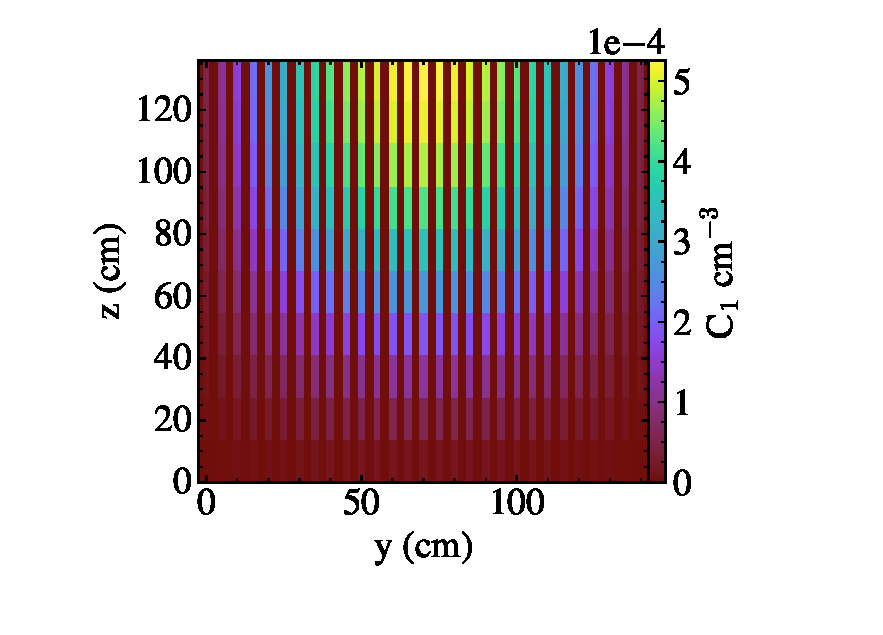
\includegraphics[width=\textwidth]{pre1.eps}
        \end{center}
        \caption{This image shows the concentration of some particularly 
        important fission-product nuclides called delayed neutron precursors.  
        The concentration of the group of longest lived precursors ($\lambda = 
        1.24\times{10}^{-2}{s}^{-1}$) peaks near the reactor outlet in this 2-D 
        axisymmetric model (r = 0 is center of core).} 
        \label{fig:pre1}
        \end{subfigure}\hfill%
        \begin{subfigure}{0.4\textwidth}
        \begin{center}
                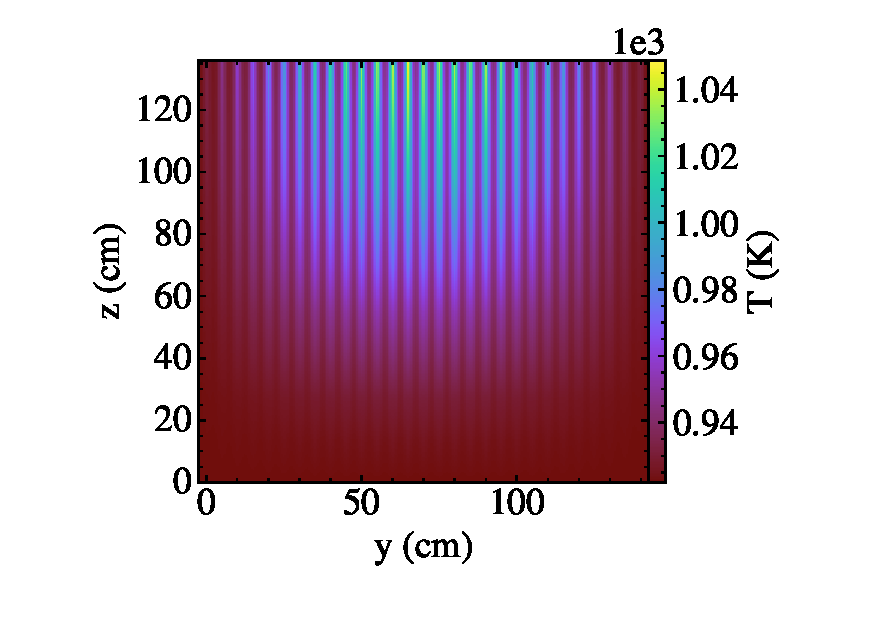
\includegraphics[width=\textwidth]{temp.eps}
        \end{center}
        \caption{This image shows the temperature in a 2-D cylindrical 
        axisymmetric model of an MSR. The reactor core temperature peaks near 
the reactor outlet in this 2-D axisymmetric model because of fuel advection (r 
= 0 is center of core).}% 
        \label{fig:temp}
        \end{subfigure}%
\end{figure}


Additionally, we have developed
an online reprocessing model, SaltProc which includes fission product removal, fissile material
separations, and refuelling for time dependent analysis of fuel-salt evolution.
This tool relies on full-core high-fidelity Monte Carlo simulations perform depletion
computations. Simulations which faithfully capture this coupling at realistic spatial and
temporal resolution are only possible with the aid of high performance
computing resources.

\textbf{This capability enables unprecidented fidelity in dynamic fuel cycle 
analysis for liquid fueled reactors.} This analysis requires thousands of full 
core simulations for relevant timescales. With Blue Waters, we accomplished 
this high fidelity fuel cycle simulation and provided the field with 
unprecedented detail in the dynamics of fuel processing for molten salt 
reactors. 

These fuel cycle simulations have occupied up to many hundreds of nodes
simultaneously and have resulted in rich datasets for use in reactor design and
analysis.  Fuel cycle dynamics and quasi-equilibrium compositions were obtained
from depletion and reprocessing simulations for a 10-year time frame. The MSBR
full-core safety analysis was performed at the initial and equilibrium fuel
salt compositions, for various reactor safety parameters such as effective
multiplication factor, neutron flux distributions, temperature coefficients,
rod worths, power and breeding distributions.

\begin{figure}[ht]
        \begin{center}
                \includegraphics[width=0.5\textwidth]{plan_view_ser.png}
        \end{center}
        \caption{High fidelity monte carlo neutron transport solutions in the
                Molten Salt Breeder Reactor (MSBR) are at the heart of fuel cycle
        analysis on Blue Waters. Above, yellow represents the fuel salt, purple 
represents the graphite moderator, and blue is the outer vessel.}
        \label{fig:plan_view}
\end{figure}

\begin{figure}[ht]
   \begin{subfigure}{.5\textwidth}
   \includegraphics[width=\textwidth]{./power_distribution.png}
        \label{fig:power_dens}
   \caption{Normalized power density}
   \end{subfigure}
   \begin{subfigure}{.5\textwidth}
          \includegraphics[width=\textwidth]{./breeding_distribution.png}
   \caption{$^{232}$Th neutron capture reaction rate normalized by total flux}
        \label{fig:breed_dens}
   \end{subfigure}
    \end{figure}

Figures~\ref{fig:keff} and \ref{fig:keff_zoomed} show the effective 
multiplication factors (criticality) obtained using SaltProc and SERPENT2. The 
criticality values were
calculated after removing fission products at varying rates 
and adding the fertile material at the end of
cycle time (3 days for this work) over the full 60 year lifetime of this 
reactor concept. This simulation demonstrated in detail how the effective multiplication
factor fluctuates significantly as a result of the batch-wise nature of this
online reprocessing strategy.

\begin{figure}[ht!]
  \centering
  \includegraphics[width=\textwidth]{keff.png}
  \caption{Effective multiplication factor dynamics for full-core MSBR
  model over a 60-year reactor operation lifetime.}
  \label{fig:keff}
\end{figure}
\begin{figure}[ht!]
  \centering
  \includegraphics[width=\textwidth]{keff_zoomed.png}
  \caption{Zoomed effective multiplication factor for 150-EFPD time interval.}
  \label{fig:keff_zoomed}
\end{figure}

First, SERPENT calculates the effective multiplication factor for the beginning
of the cycle (there is fresh fuel composition at the first step). Next, it
computes the new fuel salt composition at the end of a 3-day depletion. The
corresponding effective multiplication factor is much smaller than the previous
one. Finally, SERPENT calculates $k_{eff}$ for the depleted composition after
applying feeds and removals. The $K_{eff}$ increases accordingly since major reactor
poisons (e.g. Xe, Kr) are removed, while fresh fissile material ($^{233}$U)
from the protactinium decay tank is added.


\FloatBarrier


\section{List of publications associated with this work}

%List any publications and products (including papers in-preparation and 
%submitted, posters, and curricular materials that can be made available to the 
%community). Indicate the current state (work in progress/submitted/published). 
%If available, please include the DOI for published works.

%Highlight any keynote or other presentations that featured your work on Blue Waters.

\subsection{Publications and Products}

\begin{itemize}

               \item A. Rykhlevskii, B. R. Betzler, A. Worrall, and K. D. Huff, 
                       ``Fuel Cycle Performance of Fast Spectrum Molten Salt 
                       Reactor Designs,'' in Proceedings of Mathematics and 
                       Computation 2019, Portland, OR, 2019.
               \item G. Chee, J. W. Bae, K. D. Huff, R. R. Flanagan, and R. 
                       Fairhurst, ``Demonstration of Demand-Driven Deployment 
                       Capabilities in Cyclus,'' in Proceedings of the American 
                       Nuclear Society 2019 Global Conference, Seattle, WA, 
                       United States, September 2019.
               \item R. R. Flanagan, J. W. Bae, K. D. Huff, G. J. Chee, and R. 
                       Fairhurst, ``Methods for Automated Fuel Cycle Facility 
                       Deployment,'' in Proceedings of the American Nuclear 
                       Society 2019 Global Conference, Seattle, WA, United 
                       States, September 2019.
               \item A. Rykhlevskii and K. Huff, ``Milestone 2.1 Report: 
                       Demonstration of SaltProc,'' University of Illinois at 
                       Urbana-Champaign, Urbana, IL, Milestone Report 
                       UIUC-ARFC-2019-04 
                       \url{https://doi.org/10.5281/zenodo.3355649}, Jun. 
                       2019.
               \item G. Chee, R. Fairhurst, and K. Huff, ``Transition Scenario 
                       Demonstrations of CYCAMORE Demand Driven Deployment 
                       Capabilities,” University of Illinois at 
                       Urbana-Champaign, Urbana, IL, Technical Report 
                       UIUC-ARFC-2019-03 \url{https://doi.org/10.5281/zenodo.3354507}, Jun. 2019.  
              \item J. W. Bae, C. E. Singer, and K. D. Huff, ``Synergistic 
                      spent nuclear fuel dynamics within the European Union,'' 
                      Progress in Nuclear Energy, vol. 114, pp. 1–12, Jul. 
                      2019, \url{https://doi.org/10.1016/j.pnucene.2019.02.001}.
               \item A. Rykhlevskii, J. W. Bae, and K. D. Huff, ``Modeling and 
                simulation of online reprocessing in the thorium-fueled molten 
                salt breeder reactor,'' Annals of Nuclear Energy, vol. 128, pp. 
                366–379, Jun. 2019. 
                \url{https://doi.org/10.1016/j.anucene.2019.01.030}
        \item J. W. Bae, J. L. Peterson-Droogh, and K. D. Huff, “Standardized 
                verification of the Cyclus fuel cycle simulator,” Annals of 
                Nuclear Energy, vol. 128, pp. 288–291, Jun. 2019. 
                \url{https://doi.org/10.1016/j.anucene.2019.01.014}
        \item A. Lindsay, G. Ridley, A. Rykhlevskii, and K. Huff, 
                ``Introduction to Moltres: An application for simulation of 
                Molten Salt Reactors,'' Annals of Nuclear Energy, vol. 114, pp. 
                530–540, Apr. 2018. \url{https://doi.org/10.1016/j.anucene.2017.12.025}
        \item A. Rykhlevskii, ``Advanced online fuel reprocessing simulation 
                for Thorium-fuled Molten Salt Breeder Reactor,'' Master’s 
                thesis, University of Illinois at Urbana-Champaign, Apr. 2018. 
                \url{http://hdl.handle.net/2142/101052}
        \item A. Rykhlevskii, J. W. Bae, and K. Huff, ``arfc/saltproc: Code for 
                online reprocessing simulation of molten salt reactor with 
                external depletion solver SERPENT,'' Zenodo, Mar. 2018. 
                \url{https://doi.org/10.5281/zenodo.1306628}
        \item A. Lindsay and K. Huff, ``Moltres: finite element based 
                simulation of molten salt reactors,'' The Journal of Open 
                Source Software, vol. 3, pp. 1–2, Jan. 2018. 
                \url{https://doi.org/10.21105/joss.00298}
        \item Ridley, G., 2017. Multiphysics Analysis of Molten Salt Reactor Transients (Undergraduate Report No. UIUC-ARFC-2017-01), Advanced Reactors and Fuel Cycles Group Report Series. University of Illinois at Urbana-Champaign, Urbana, IL. \url{https://github.com/arfc/publications/tree/2017-ridley-msrTransients}.
        \item A. Rykhlevskii, A. Lindsay, and K. D. Huff, ``Full-core analysis of thorium-fueled Molten Salt Breeder Reactor using the SERPENT 2 Monte Carlo code,'' in Transactions of the American Nuclear Society, (Washington, DC, United States), American Nuclear Society, Nov. 2017.
        \item G. Ridley, A. Lindsay, and K. Huff, ``An Introduction to Moltres, an MSR Multiphysics Code,'' in Transactions of the American Nuclear Society, (Washington D.C.), American Nuclear Society, Oct. 2017.
        \item G. Ridley, A. Lindsay, M. Turk, and K. Huff, ``Multiphysics Analysis of Molten Salt Reactor Transients,'' Undergraduate Report UIUC-ARFC-2017-01, University of Illinois at Urbana-Champaign, Urbana, IL, Aug. 2017. DOI 10.5281/zenodo.1145437.
	\item Lindsay, A., Huff, K., Rykhlevskii, A., 2017. arfc/moltres: Initial Moltres release. Zotero. doi:\url{dx.doi.org/10.5281/zenodo.801823}.
\end{itemize}

\subsection{Highlighted Keynotes and Media}
PI Huff gave two keynote talks in 2017. One was to PyCon 2017, with an audience of over 3000 people. The 
second was at SciPy 2017, with an audience of 700 people. Each keynote 
mentioned affiliation with NCSA, support as a Blue Waters Professor, and 
the work being conducted on Blue Waters in the ARFC group. 


\begin{itemize}
\item Kathryn Huff, ``Academic Open Source'' Scientific Python Conference 
(SciPy2017), Austin, TX. July 12, 2017.  
Presentation: \url{http://katyhuff.github.io/2017-07-12-scipy}. Video: 
\url{https://www.youtube.com/watch?v=Nqzvnqg4OJ8}.
\item Kathryn Huff, ``Do it for Science'' Python Conference (PyCon2017),
Portland, OR, May 20, 2017. Presentation: \url{http://katyhuff.github.io/2017-05-20-pycon}.
Video: \url{https://www.youtube.com/watch?v=kaGS4YXwciQ}.
\end{itemize}

Similarly, Prof. Huff was featured in the media recently. These items 
feature discussion of nuclear engineering enabled by Blue Waters and mention 
Blue Waters specifcally:

\begin{itemize}
        \item B. Kugelmass, ``Katy Huff, University of Illinois on Apple 
                Podcasts,'' Titans Of Nuclear | Interviewing World Experts on 
                Nuclear Energy, Apple Podcasts, Urbana, IL, April 2019. 
                \url{https://www.titansofnuclear.com/katyhuff}
        \item S. Mumm, ``NPRE researchers to investigate load-following 
                capabilities for molten salt reactors | NPRE Illinois,'' 
                Nuclear, Plasma, and Radiological Engineering News, June 26, 
                2018. \url{https://npre.illinois.edu/news/npre-researchers-investigate-load-following-capabilities-molten-salt-reactors}
        \item Hugo Bowne-Anderson, ``Data Science, Nuclear Engineering and the 
                Open Source (with Katy Huff),'' Data Framed, Data Camp, New 
                York, NY, USA, March 5, 2018. \url{https://www.datacamp.com/community/podcast/data-science-nuclear-engineering}
        \item S. Hacksworth, ``Nuclear Engineering Programs with Dr. Kathryn 
                Huff,'' Yes College Podcast, YesCollege.com, Chicago, IL, 
                United States, February 15, 2018. \url{https://yescollege.com/episode/kathryn-huff/}
\end{itemize}

\subsection{Highlighted Presentations} The work conducted on Blue Waters using 
Moltres appeared in detail within three presentations during the course of the 
allocation. 

\begin{itemize} 
        \item Kathryn D. Huff, ``Sustaining Student Software,'' poster 
                presented at  
                the Society of Industrial and Applied 
                Mathematics (SIAM) Computational Science and Engineering 
                (CSE)SIAM CSE: Minisymposerium: Software Productivity and 
                Sustainability for CSE and Data Science, Spokane, WA, February 25, 2019.
                Presentation: 
                \url{https://doi.org/10.6084/m9.figshare.7768349.v1}
        \item Kathryn D. Huff, ``Neutron Kinetics in Liquid-Fueled Nuclear 
                Reactors,'' presented at 
                the Society of Industrial and Applied 
                Mathematics (SIAM) Computational Science and Engineering 
                (CSE)SIAM CSE: Computational Methods of Kinetics of Gases and 
                Plasmas Minisymposium, Spokane, WA, February 25, 2019.
                Presentation: \url{http://arfc.github.io/pres/2019-02-20-purdue.pdf}
        \item Andrei Rykhlevskii, ``Simulation of Molten Salt Reactors with 
                Moltres,'' presented at the SIAM CSE 2019, Spokane, WA, 
                February 26, 2019. 
                Presentation: \url{http://arfc.github.io/pres/2019-02-26-rykhlevskii-siam.pdf}
        \item Andrei Rykhlevskii, ``Fuel Cycle Performance of Fast Spectrum Molten Salt Reactor Designs,'' presented at the NESLS Poster Session, Oak Ridge, TN, United States, August 6, 2018.  Presentation: \url{http://arfc.github.io/pres/2018-08-08-fs_msrs_poster.pdf}

        \item Kathryn Huff, ``Doing Our Best: Approaches for Scientific 
                Computing,'' presented at the Institute for Advanced 
                Computational Science Seminar, Stony Brook University, November 
                8, 2018. Presentation: 
                \url{https://katyhuff.github.io/2018-11-08-iacs/} 
        \item Andrei Rykhlevskii, ``Computational Tools for Molten Salt Reactor 
                Simulation,'' presented at the Blue Waters Symposium, Sun 
                River, OR. June 4, 2018. Presentation: 
                \url{http://arfc.github.io/pres/2018-04-07-comp-tools-msr.pdf}
        \item Kathryn D. Huff, ``Modeling and Simulation at Disparate Scales: 
                Molten Salt Reactor Physics and International Fuel Cycle 
                Transitions,'' presented at the NERS Colloquium, Ann Arbor, MI. 
                February 16, 2018. Presentation: 
                \url{https://katyhuff.github.io/2018-02-16-ners}
        \item Alexander Lindsay and Kathryn Huff, ``Moltres: a MOOSE 
                Application for Simulation of MSRs.'' Workshop on Multi-physics 
                Modeling and Simulation of Molten Salt Reactors, Berkeley, 
                CA.June 15, 2017. Presentation: 
        \url{arfc.npre.illinois.edu/img/pres/2017-06-15-msr-pres.pdf}. 
        \item Kathryn Huff, ``Modeling and Simulation of Advanced Reactors and 
                Fuel Cycles,'' Invited Seminar, UC Davis Mechanical and 
                Aerospace Engineering Seminar, Davis, CA. April 20, 2017. 
                Presentation: \url{http://katyhuff.github.io/2017-04-20-davis}. 
                Video: 
                \url{https://www.youtube.com/watch?v=YqTxZC1i-B0#t=6m28s}
        \item Kathryn Huff, ``Advanced Nuclear Reactors and Fuel Cycles: 
                Simulation of Multiple Physics at Disparate Scales'' 
                Computational Science and Engineering Seminar Series, 1030 
                National Center for Supercomputing Applications, Urbana, IL. 
                February 2, 2017. Presentation: 
                \url{http://katyhuff.github.io/2017-02-02-cse}.  Video: 
                \url{https://www.youtube.com/watch?v=fWlUW_CFo3M}.
        \item Gavin Ridley. ``Transient Simulations of Next Generation Nuclear 
                Reactors.'' Illinois Summer Research Symposium, Session: 
                Improving Big Data Algorithms for Food and Energy Security, 
                Urbana, IL. July 21, 2017 (Awarded Honorable Mention for 
                Outstanding Oral Presentation). \url{http://www.grad.illinois.edu/sites/default/files/PDFs/ISRS-program-booklet-2017.pdf}
\end{itemize}

\section{Plan for Blue Waters use in 2019-2020}

The development of the Moltres software  began in September 2016 and has now been
demonstrated on hundreds of nodes on Blue Waters. We haved scaled that up to
include very (spatially) large reactor core simulations of the Molten Salt 
Breeder Reactor design and the Transatomic Power reactor. This year we will 
continue to emphasize transient accident scenarios (Moltres) and fuel salt 
reprocessing analysis (SaltProc) in both of these reactor designs. 
Additionally, extensions to Moltres will be developed based on high fidelity 
Nek5000 simulations capturing vortical flow regimes in MSRs.  These 
simulations are in  progress.

\paragraph{For the remainder of 2019} I would like to request an increase in my 
current allocation, which will be spent soon. My current allocation has been 
spent more quickly than I anticipated (it was 80\% spent in August). I expect we will need an additional 
30,000 node hours beyond the existing allocation. Figure 
\ref{fig:2019-additional} indicates the expected usage of Blue Waters in my 
group in the final quarter of 2019.


\begin{figure}[htbp!]
\begin{center}
        \includegraphics[width=\textwidth]{bw-usage-2019-additional.png}
\end{center}
\caption{Planned project schedule for molten salt reactor related activities in 
the final quarter of 2019. An additional 30,000 node hours are requested for 
        this period, if available.}
\label{fig:2019-additional}
\end{figure}

\paragraph{For 2020} I would like to request 200,000 node hours, total, with a 
distribution of use that is weighted toward the front end of the year. 
Figure \ref{fig:bw-usage-2020} reflects the planned work in 2020 in my group as 
well as a distribution of usage per month and quarter.

\begin{figure}[htbp!]
\begin{center}
        \includegraphics[width=\textwidth]{bw-usage-2020.png}
\end{center}
\caption{Planned project schedule for molten salt reactor related activities in 
2020. A total request of 200,000 node hours are requested for 2020.}
\label{fig:bw-usage-2020}
\end{figure}

The following updates will continue to support our research 
productivity this year. 

\begin{itemize}
        \item \textbf{Larger Scale Problems} The software we developed in house 
                (moltres) is now capable of 3D simulation and can be used by 
                many students. Accordingly, we expect this portion of our 
                activity to be strong this year. Additionally, high fidelity 
                Nek5000 \cite{fischer_petascale_2008} simulations of complex flow regions in MSRs will be 
                conducted to capture vortical flows. This new activity will be 
                computationally expensive, but will yield powerful new insights 
                with regard to reactor safety in advanced nuclear reactors.
        \item \textbf{Monte-Carlo Cross-Section Generation} The ARFC group 
                began working with monte-carlo software for cross section 
                generation last year. The Serpent 2 software is fully parallelizable, very 
                memory intensive, and produces very high fidelity results. 
                We will continue this activity in the remainder of 2019 and the computational 
                intensity of our work will remain stable.
\item \textbf{Group Size} The number of graduate students in the Advanced Reactors and Fuel Cycles
                group rose to 9 in 2018 and will remain approximately this size 
                through 2020.
        \item \textbf{Expansion into Agent Based Modeling} The scope of the 
                work within ARFC will continue to include some capacity 
                computing work. While this is not the bulk of ARFC work, we 
                have a project in statistical optimization methods for agent 
                based modeling (the Cyclus application 
                \cite{huff_fundamental_2016}) that benefits
                from a few hundreds or thousands of independent single-node 
                runs. This work, including transition scenarios 
                \cite{bae_synergistic_2019,bae_standardized_2019}, is moving toward predictive algorithms informed 
                by machine learning \cite{bae_deep_2019}.
\end{itemize}

\paragraph{System nodes needed per run:} 20 - 2,000. Many simulations will be 
run on 10-200 nodes, while a few much larger simulations will be run on 5,000 
nodes. Larger runs, particularly with Nek5000 and Moltres are possible this year.
\paragraph{Anticipated memory usage:} Some Nek5000 simulations may require the 
high memory nodes..
\paragraph{Expected numerical operations:} Unknown.
\paragraph{Expected local and remote memory accesses:} Unknown. 
\paragraph{Total Node Hours:} Approximately 200,000 node hours.
\paragraph{Anticipated data transfer:} Data transfer will be in the ``few 
gigabytes'' per run for most runs. Large runs may be in the ``tens of 
gigabytes'' and some on the order of 100GB.

%Describe the Blue Waters resources required for next year. This description 
%should include the number of system nodes needed for your runs, the 
%anticipated actual memory usage, the expected numbers of each major class of 
%arithmetic and logical operation, the expected numbers of local and remote 
%memory accesses, the total number of node-hours required, the anticipated 
%input and output requirements, the amount of data that you anticipate 
%transferring to or from the Blue Waters enclave, the amount and type of 
%storage required and any other system resource needs that you anticipate

%For assistance in computing node hours for Blue Waters see: 
%https://bluewaters.ncsa.illinois.edu/node\_core\_comparison

%For a description of the default storage quotas see: 
%https://bluewaters.ncsa.illinois.edu/storage. If your project will require 
%storage limits that exceed the standard quotas, provide a justification in 
%support of your request.


\subsection{Usage Schedule:} See Figures \ref{fig:2019-additional} and 
\ref{fig:bw-usage-2020}.
%Provide an estimated Blue Waters usage schedule. The estimate should be per 
%quarter and may be represented as a percent of the requested allocation (e.g. 
%Q1: 10\%, Q2: 20\%, Q3: 50\%, Q4: 20\%).

 

%The report should be submitted as a PDF file. There are no specific formatting 
%instructions. It is recommended to include visualizations, charts and other 
%images in the document to help illustrate the results. 

%If you have questions, please contact Jay Roloff at cesc@ncsa.illinois.edu or 
%the Blue Waters support staff at help+bw@ncsa.illinois.edu.
\subsection{End-of-life Data Handling}
As we have in the past, our work will emphasize immediate data transfer and 
archiving for all simulation results. This continuous data handling allows our 
group assurance that the final closeout of the Blue Waters machine will not 
impact our ability to access our data. We typically use archival resources on 
our local storage as well as the Illinois Data Bank and the Zenodo platform. 

\pagebreak
\bibliographystyle{ieeetr}
\bibliography{2020-bw-report}


\end{document}


